\chapter{Fuente Regulada Serie}

\hspace{10pt}
El  circuito de la figura \ref{lab4_1} corresponde a una Fuente
Regulada Serie con limitación de corriente. Realizar el diseño de la
Fuente asegurando una tensión regulada de salida de 12V, para una
tensión continua de entrada de 18V, siendo la corriente máxima de
salida de 650mA

Armar la fuente en un circuito de prueba y realizar las siguientes
mediciones:
\begin{enumerate}
	\item Variar $R_4$, sin carga, y verificar que $V_o$ cambia
	dentro del rango deseado, dejándolo ajustado en 12V. Verificar que
	las tensiones y corrientes del circuito son las esperadas para esta
	condición.
	\item Conectar una resistencia de carga variable
	proporcionada por la cátedra y tomar los datos para trazar la curva
	de salida tensión-corriente (regulación de carga). Tomar valores
	cada 100mA, hasta llegar al corto circuito.
	\item Cambiar la protección contra sobrecargas por otra con repliegue (ver figura \ref{lab4_2}). Calcular $R_s$ y
	las resistencias correspondientes al divisor de base del transistor
	$Q_4$. Para una corriente máxima $I_{Lmax}=1A $ y una corriente de
	corto circuito $I_{FB}=300mA$.
	\item Ajustar la tensión de salida a 10 V. Alimentar la fuente regulada con un rectificador de onda
	completa provisto por la cátedra. Evaluar el factor de regulación
	midiendo la tensión de ripple a la entrada y a la salida de la
	fuente regulada para un estado de carga de 200mA . Para esta
	medición utilizar un voltímetro, desacoplándolo en continua mediante
	un capacitor.
	\begin{equation}
		S_v= \frac{\displaystyle \frac{\displaystyle \Delta
				V_o}{\displaystyle V_o}}{\displaystyle \frac{\displaystyle \Delta
				V_i}{\displaystyle V_i}}100
	\end{equation}
	
	\item Realizar un informe escrito completo.
	
	Instrumental disponible: Fuente regulada variable de entrada con medición de
	tensión y corriente, Multímetro digital, resistencia variable de
	potencia.
\end{enumerate}

\begin{figure}[h]
	\centering
	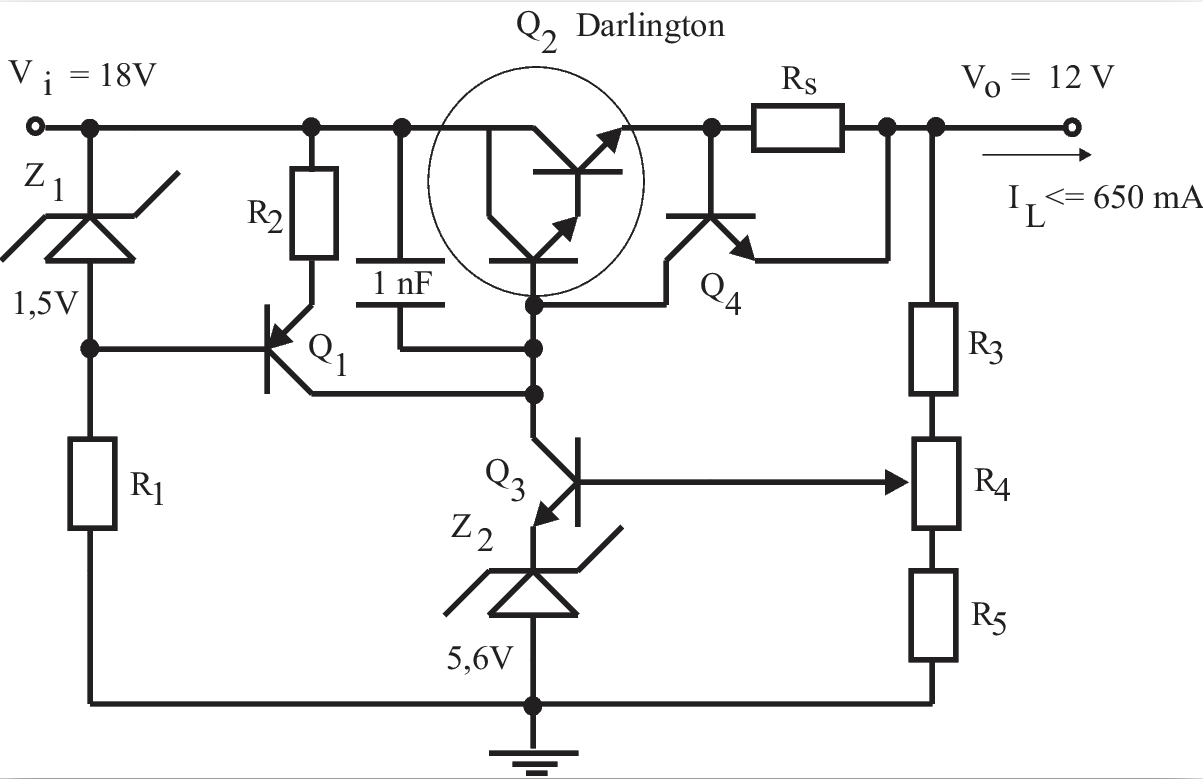
\includegraphics[width=0.8\linewidth]{figuras/lab4_1.png}\\
	\caption{}\label{lab4_1}
\end{figure}

\begin{figure}[h]
	\centering
	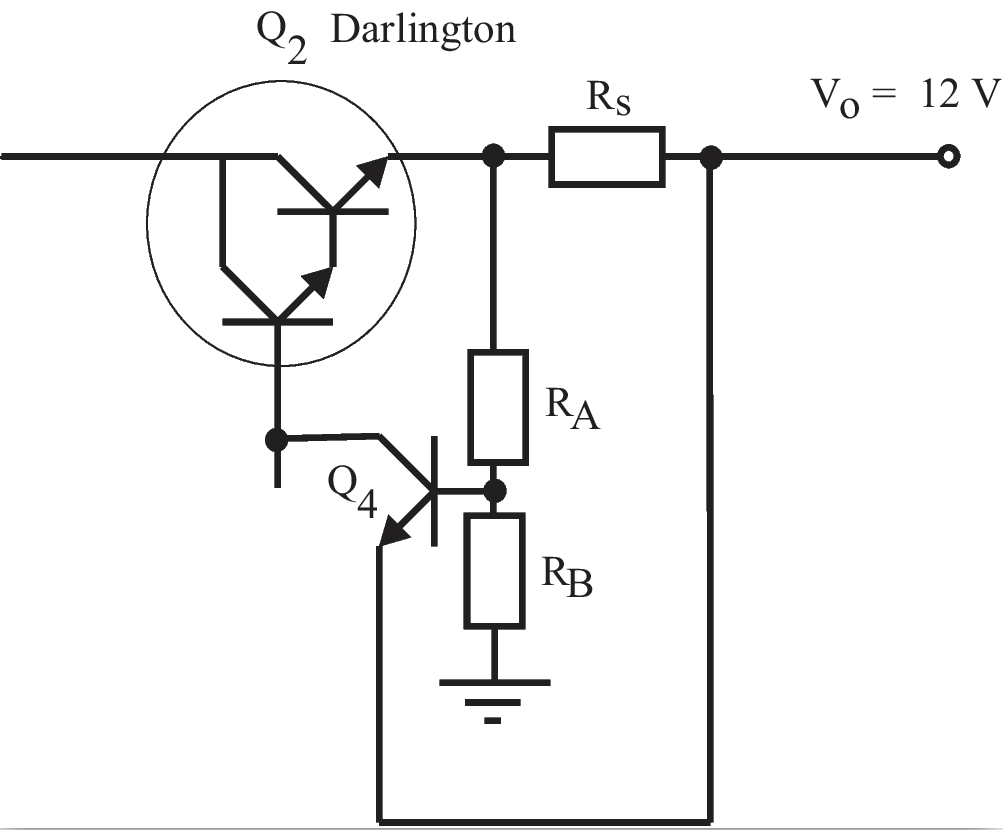
\includegraphics[width=0.8\linewidth]{figuras/lab4_2.png}\\
	\caption{}\label{lab4_2}
\end{figure}
\end{document}